%!TEX TS-program = Arara
% arara: pdflatex: {shell: yes}
% arara: biber
% arara: pdflatex: {shell: yes}
\documentclass[12pt, ngerman, parskip=half]{scrreprt}

%!TEX TS-program = Arara
%!TeX root=Hauptdokument.tex
\usepackage[T1]{fontenc}
\usepackage{booktabs}
\usepackage{babel}
\usepackage{graphicx}
\usepackage{csquotes}
\usepackage{paralist}
\usepackage{xcolor}

\usepackage{prettyref}
% for prettyref
\newrefformat{cha}{Kapitel \ref{#1}}
\newrefformat{sec}{Abschnitt \ref{#1}}
\newrefformat{tab}{Tabelle \ref{#1} auf Seite \pageref{#1}}
\newrefformat{fig}{Bild \ref{#1} auf Seite \pageref{#1}}


\usepackage[style=authoryear-icomp, backend=biber,natbib]{biblatex}
\addbibresource{Literaturverzeichnis.bib}

\usepackage{blindtext}

\usepackage{subcaption}

\usepackage{uni-titlepage}

\author{Zefram Cochrane}
\title{Reisen in Überlichtgeschwindigkeit}
\date{\today}
\place{Köln}
\extratitle{extratitle} % Schmutztitel
\frontispiece{frontispiece} % Bildertitel, https://de.wikipedia.org/wiki/Frontispiz#/media/Datei:Cl%C3%BCver-introductio-1686-1.jpg
\titlehead{Deutsches Zentrum für Luft- und Raumfahrt}
\uppertitleback{uppertitleback}
\lowertitleback{lowertitleback}
\dedication{dedication}
\faculty{Fakultät für Quantenreisen}
\chair{Prof. Dr. Daniel Düsentrieb}
\professor{professor}
\duration{2080--2095}
\referee{Dagobert Duck}
\subject{Dissertation}
%\student{student}
\discipline{discipline}
\matriculationnumber{matriculationnumber}
\advisor{Prof. Dr. Daniel Düsentrieb}
\TitlePageStyle{KIT}

\usepackage{hyperref}
\hypersetup{
    bookmarks=true,                     % show bookmarks bar
    unicode=false,                      % non - Latin characters in Acrobat’s bookmarks
    pdftoolbar=true,                        % show Acrobat’s toolbar
    pdfmenubar=true,                        % show Acrobat’s menu
    pdffitwindow=false,                 % window fit to page when opened
    pdfstartview={FitH},                    % fits the width of the page to the window
    pdftitle={My title},                        % title
    pdfauthor={Author},                 % author
    pdfsubject={Subject},                   % subject of the document
    pdfcreator={Creator},                   % creator of the document
    pdfproducer={Producer},             % producer of the document
    pdfkeywords={keyword1, key2, key3},   % list of keywords
    pdfnewwindow=true,                  % links in new window
    colorlinks=true,                        % false: boxed links; true: colored links
    linkcolor=red,                          % color of internal links
    filecolor=cyan,                     % color of file links
    citecolor=green,                     % color of file links
    urlcolor=magenta                        % color of external links
}


\usepackage[style=authoryear, backend=biber]{biblatex}
\addbibresource{Literaturverzeichnis.bib}

\usepackage{uni-titlepage}
\author{Uwe Ziegenhagen}
\title{Dissertation}
\date{22.03.2022}
\place{Köln}
\advisor{Daniel Düsentrieb}

\TitlePageStyle{TU-DD}

\begin{document}
%
\begin{titlepage}
\textbf{\large Deutsches Zentrum für Luft- und Raumfahrt}\vspace*{5cm}

\begin{center}
\huge \textbf{Dissertation} \\  \textbf{zum Dr. Ing.} 
\end{center}\vspace*{-1cm}

\begin{center}
\huge \textbf{\enquote{Einstein und das Bose-Kondensat}}
\end{center}\vspace*{5cm}


vorgelegt von 

Max Mustermann \newline Matrikelnummer 123456

\vfill
Erstgutachter: Daniel Düsentrieb \newline
Zweitgutachter: Dagobert Duck

\end{titlepage}
\maketitle

\listoffigures

\listoftables

\tableofcontents

%!TeX root=Hauptdokument.tex
\chapter{Einleitung}
\section{Literatur}

\blindtext[20]


\begin{figure}
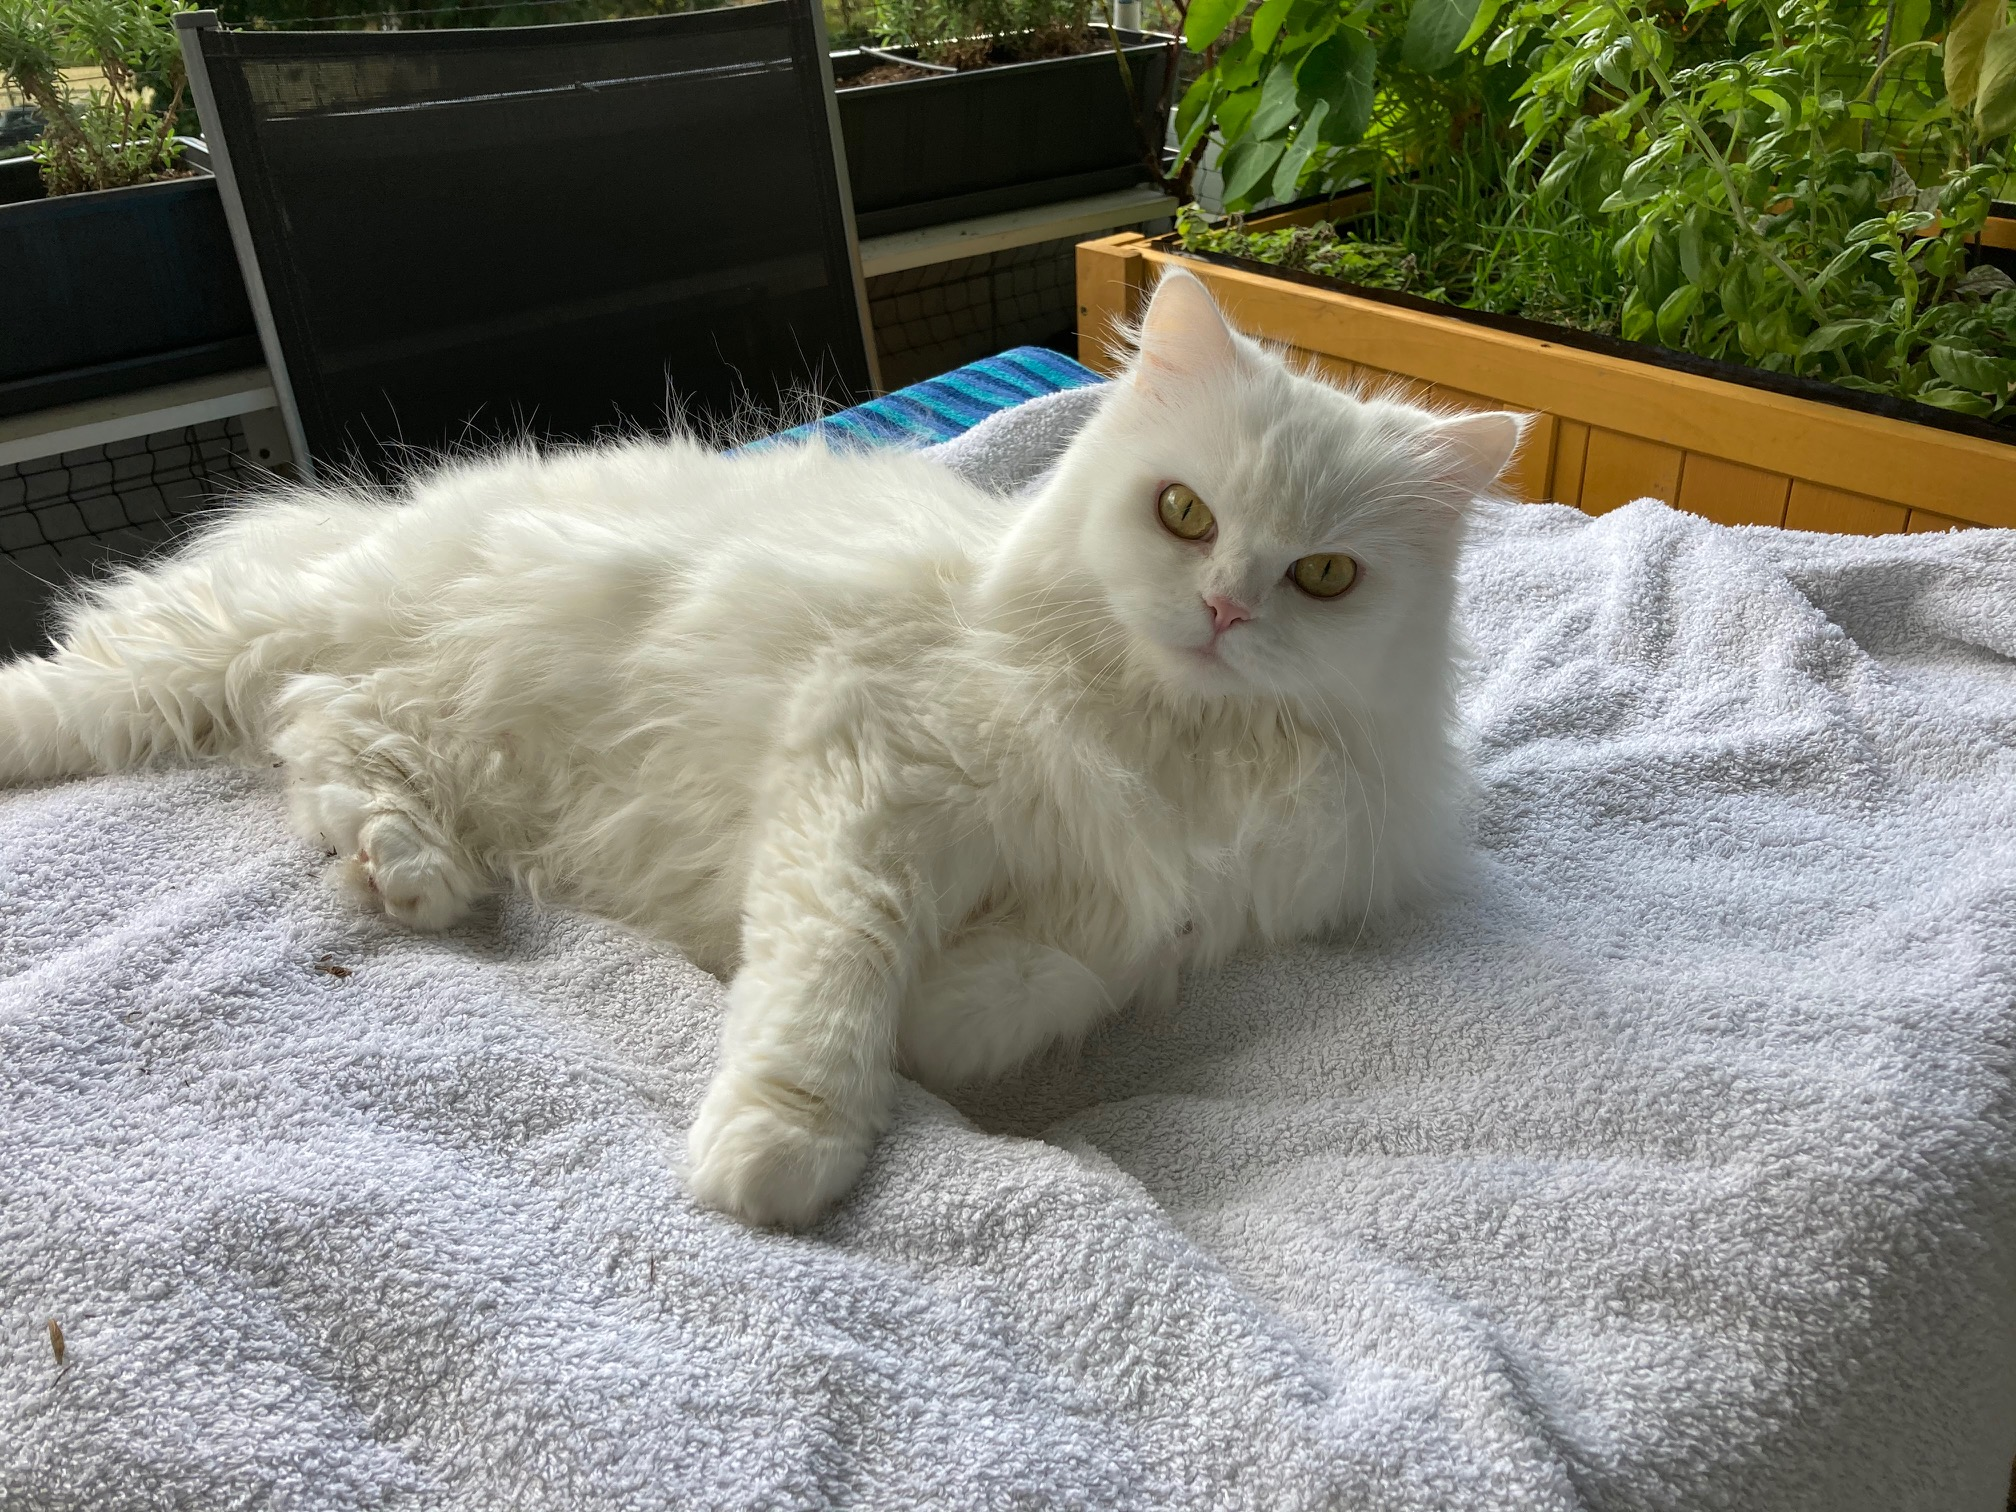
\includegraphics[width=\textwidth]{Bilder/Katze1}
\caption{Meine Miezekatze}\label{fig:katze1}
\end{figure}

% per \include einbinden
% führt vor dem Einfügen ein \clearpage aus
% das sorgt dafür, dass Floatobjekte gesetzt werden


%!TeX root=Hauptdokument.tex
\chapter{Hauptteil}
\section{Ergebnisse der Forschung}

\blindtext[20]


\blindtext[20]


% per \include einbinden
% führt vor dem Einfügen ein \clearpage aus
% das sorgt dafür, dass Floatobjekte gesetzt werden


\nocite{*}
\printbibliography[title={Bücher},type=book]

\printbibliography[title={Online-Quellen},type=online]


\end{document}